\chapter{Background}
Others have approached the objectives highlighted above in the form of Trail Running Applications, and Recommender systems. This project is an amalgamation of these topic areas, offering inspiration that will help advise the approach taken in the project.

\section{Trail Running Applications} \label{sec:TrailRunningApplications}
Many applications provide the functionality to support trail running. They are all established on the same principles of providing an interface that allows their respective users to create trails. However, each of them also has moderately different and extra services tailored around the sub-domain they are approaching.

\subsubsection{Strava}
Strava\footnote{\url{https://www.strava.com}} is a popular application that provides trail running services to its users with its website and mobile application.  The primary focus is fitness and competition.  It does this by allowing users to upload GPS data and recorded times of runs they have performed on a trail.  These details are used populate leaderboards and generate rankings for trails.

\begin{figure}[ht]
    \centering
    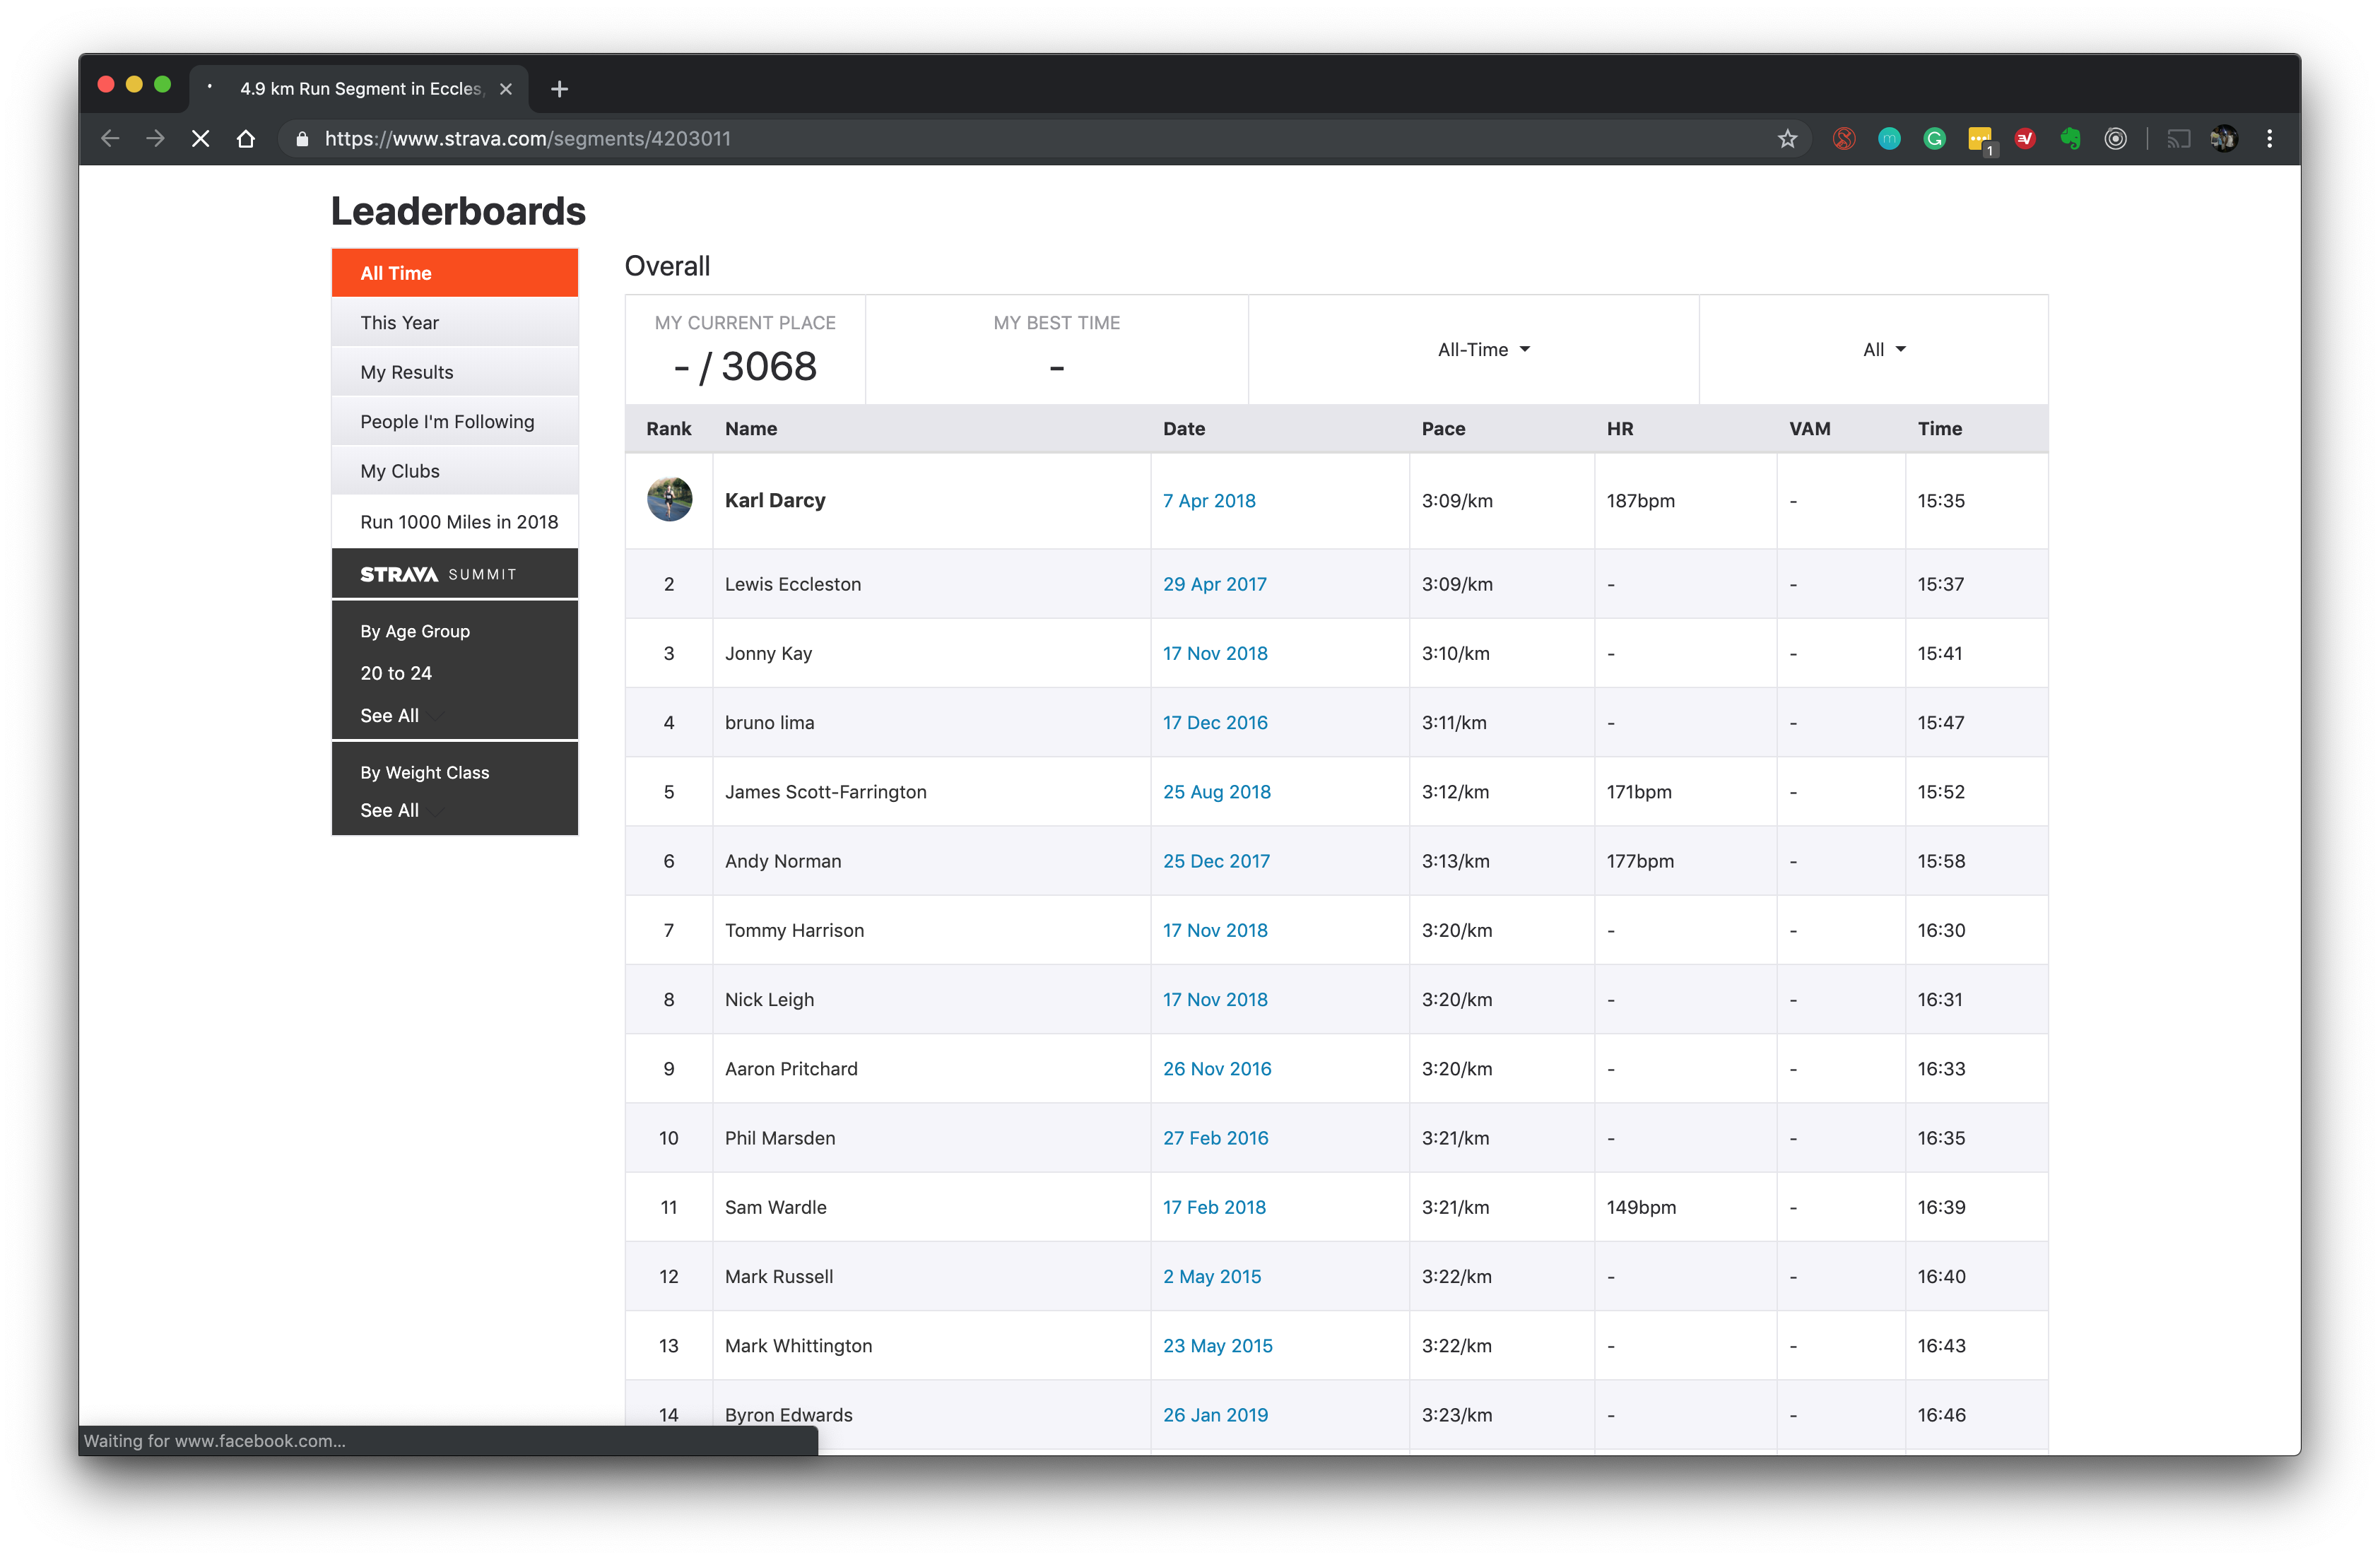
\includegraphics[width=\textwidth]{strava-leaderboards.png}
    \caption{An example of a Strava leaderboards with times from different user who ran the trail}
    \label{fig:stravaLeaderboards}
\end{figure}

\subsubsection{All Trails}
All Trails\footnote{\url{https://www.alltrails.com/}} is more concentrated on outdoor trails and exploration.  With detailed maps on outdoor paths and information on trail details such as the type of terrain, the difficulty of the trail and other types of information, and an extensive collection of hand-curated trails, its users have a wealth of choices and details to make well-informed conclusions.

\subsubsection{Ordnance Survey Maps} 
Ordnance Survey (OS) is the British national mapping agency that provides highly accurate maps of the United Kingdom \cite{wiki:OrdinanceSurvey}.  They offer a range of products such as maps and data for organizations to use.  OS Maps\footnote{\url{https://osmaps.ordnancesurvey.co.uk}} is one such product that allows users to plan and discover trails in the United Kingdom.  The main advantage of OS Maps is its extraordinarily detailed and exact map information, including paths, contours, and places of interests.


All the applications described above have above provide functionalities to create trails. They all provide a Map Interface that allows users to create trails by clicking on points on the map and connecting the points with a line that snaps to the nearest path (see figure \ref{fig:osMapsEditor}. They include searches, maps, and details on trails to help their users find what type of trail they wish to use. However, they all fail at giving personalised trails to each user. Although they use location information (trails in the user's immediate area), they do not use any information retrieval techniques to get tailored trails to each user, also known as Recommender Systems explained in section \ref{sec:RecSystems}

\begin{figure}[ht]
    \centering
    \includegraphics[width=\textwidth]{images/os-maps-editor.png}
    \caption{OS Maps trail editor that allows user to create trails by clicking on points on the map}
    \label{fig:osMapsEditor}
\end{figure}

\section{Recommender Systems} \label{sec:RecSystems}
Recommender systems are a type of Information Filtering Systems that provide suggestions that are appropriate to a user \cite{ricci2011introduction}.  Recommender systems arose as a solution to the problem of too many options, especially with the age of the Internet \cite{rishabh2019recommender}.  By trying to predict each users preferences, the system can generate a ranked list of items that are appropriate to each specific user.  The term "item" can refer to almost any product or service that requires a user’s choice. We can see  Recommender Systems in most areas such as,  movies,  products, news, people and so on.

\subsection{Why Recommender Systems} \label{subsec:WhyRecSystems}
In 1896, the Italian Economist Vilfredo Pareto proposed a theory that for events, 80\% of the effects, come from 20\% of the causes \cite{sanders1987pareto}. This theory is known as the Pareto Principle and is more commonly know as the 80/20 rule. Traditionally, this rule is a popular maxim in business and strategy management, based on the idea that 80\% of sales can be generated by 20\% of the items being offered, commonly referred to as the "best selling items".

However, in a 2004 article in \textbf{Wired} Magazine\footnote{https://www.wired.co.uk/}, Chris Anderson observed that on the internet, businesses can be more profitable by offering a larger number of niche, hard-to-find products \cite{brynjolfsson2011goodbye}. This phenomenon was coined \textbf{the Long Tail Effect}, further discussed in Chris Anderson's book \textit{"The Long Tail: Why the Future of Business Is Selling Less of More"} \cite{anderson2006long}. He explains. This new trend is is due to the the improvement in technology that enables users to search and discover more easily. It especially was strengthened by the advent of Recommender Systems. By offering more personalised items to users, we can expose users to these hard-to-find items that would have been apparent in on a popularity list. Proof of the advantages Recommender Systems offer can be seen by the major companies that take advantage of these systems.


\subsubsection{Amazon} 
Amazon is a behemoth multi-billion dollar online retail company. According to Statista, in 2018, they generated 232.89 billion dollars\footnote{https://www.statista.com/statistics/266282/annual-net-revenue-of-amazoncom/}. In a 2013 article by Mckinsey \& Company, 35\% of Amazon's revenue comes from its recommendation System. 

\subsubsection{Netflix}
Netflix is an online video streaming platform that offers thousands of TV Series and Movies to it's millions of users. Netflix uses a Recommender System not only to personalise the videos offered to the user, but also the artwork that is used as the thumbnail\footnote{a cover image for a video} for the video \cite{josefina2018netflix}.

These are just a few examples of platforms that benefit from Recommender systems \cite{polatidis2013recommender}.

\subsection{Machine Learning Approach}
Machine Learning is a study of Artificial Intelligence that uses algorithms and models to enable computer systems learn how to perform tasks using data without the need for explicit instructions to be given \cite{michie1994machine}. Machine learning models are used for a variety of tasks such as classification\footnote{differentiation between items}, facial recognition, regression analysis and so on.

Regression Analysis is a set of techniques that discover relationships between variables in data \cite{chatterjee2015regression}. By trying to find a best fit between variables in data, you can discover the relationship between them and also predict values for new variables. Regression analysis can also be described as a predictive analysis. In this sense, Recommender Systems can be seen as a Regression Analysis problem, as the system try's to predict a user's predicted rating of an Item. Hence we have a means to creating a Recommender System using Machine learning Methods.

\subsection{The Netflix Prize}

\section{GraphQL over REST}
Web applications consists of two main parts: the client, which contains the user interface the user interacts with, and the server, which provides the resources needed to be consumed by the client. In recent years, \acrfull{rest}, more commonly known as  has quickly been adopted in industry as the standard for creating servers \cite{guy2015rest}. They allow the client to access the resources provided in the server using stateless operations with the use of URLs. However one of the main problems with \acrshort{rest} is it's lack of flexibility. The resources in \acrshort{rest}, exposed via URLs defined by the server and not the client. This can lead to problems of over-fetching when the client tries to retrieve data from the server, an example is shown \autoref{fig:restProblem}.

\begin{figure}[ht]
    \centering
    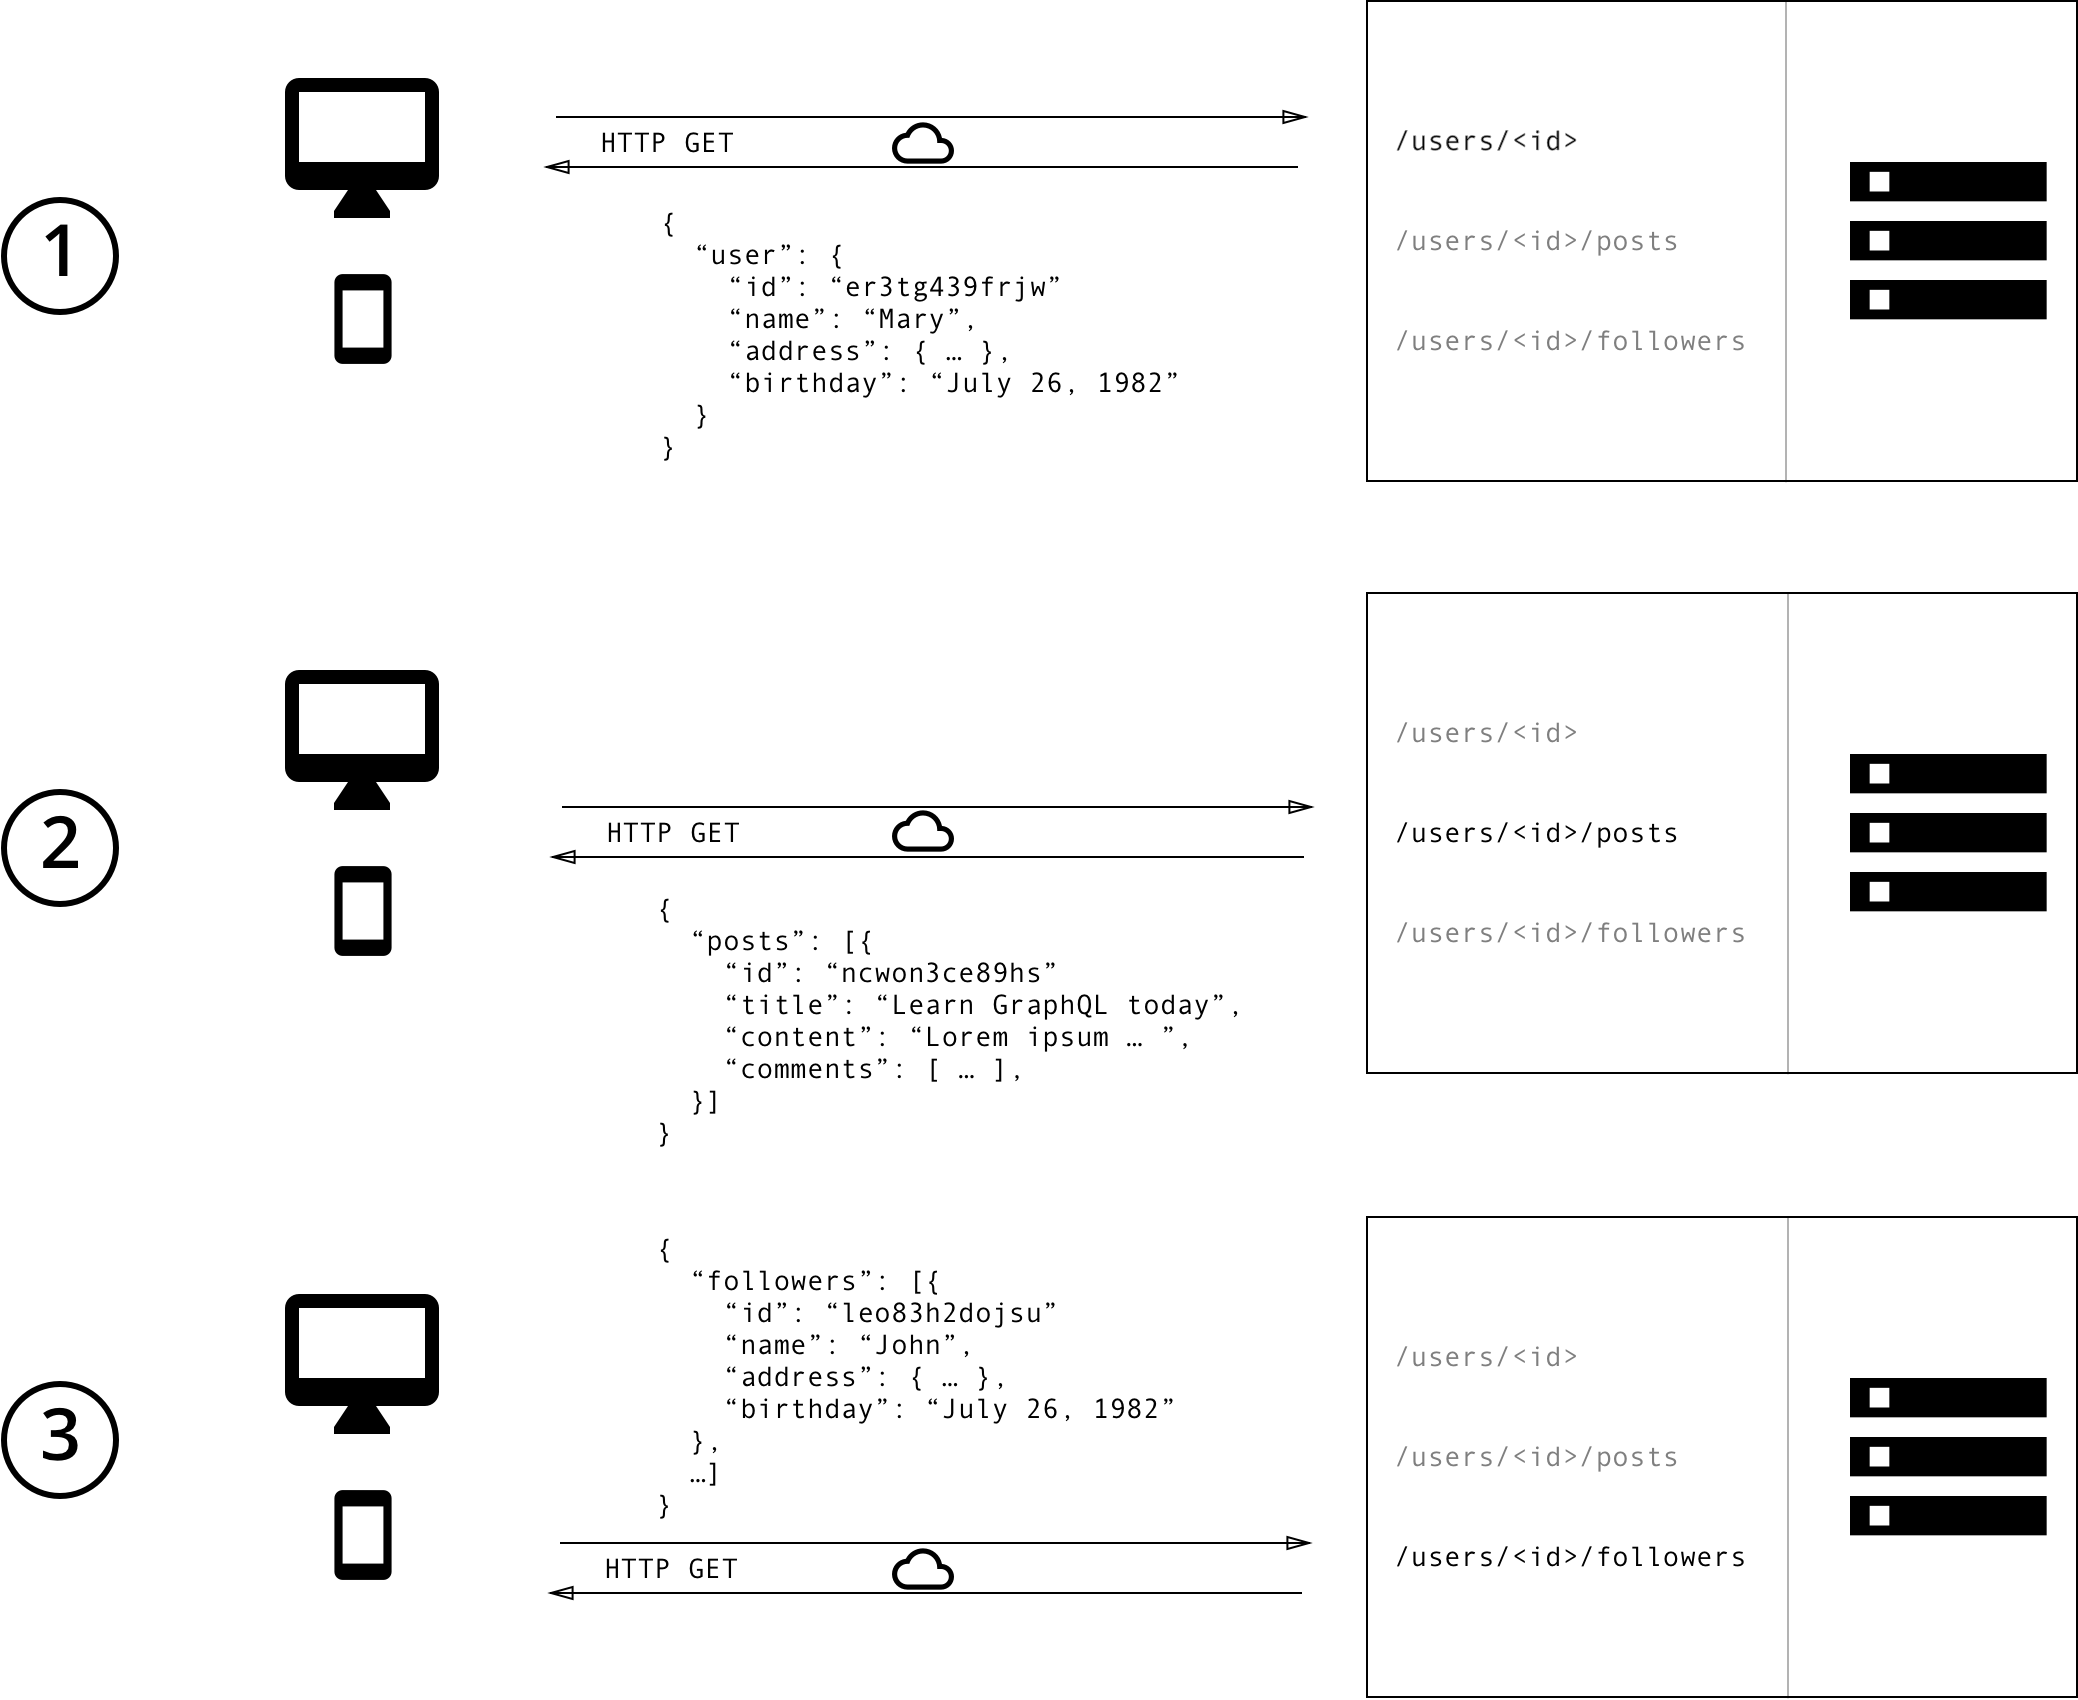
\includegraphics[width=\textwidth]{problems-with-rest.png}
    \caption{The problem with over-fetching with REST API's}
    \label{fig:restProblem}
\end{figure}

GraphQL was introduced as a solution to the shortcommings with \acrshort{rest} GraphQL is a query language for APIs and a runtime for fulfilling those queries with your existing data \cite{graphQl}. Created by Facebook in 2012 and then open sourced in 2015. It was created as a solution to the issues that the standard \acrshort{rest} API's that. Like \acrshort{rest}, GraphQL is used to expose resources to the client. However, with GraphQL, the client defines the structure of the data that is required \cite{howToGraphQl}, eliminating the problem of over-fetching as shown in figure \autoref{fig:graphqlFix}.

\begin{figure}[ht]
    \centering
    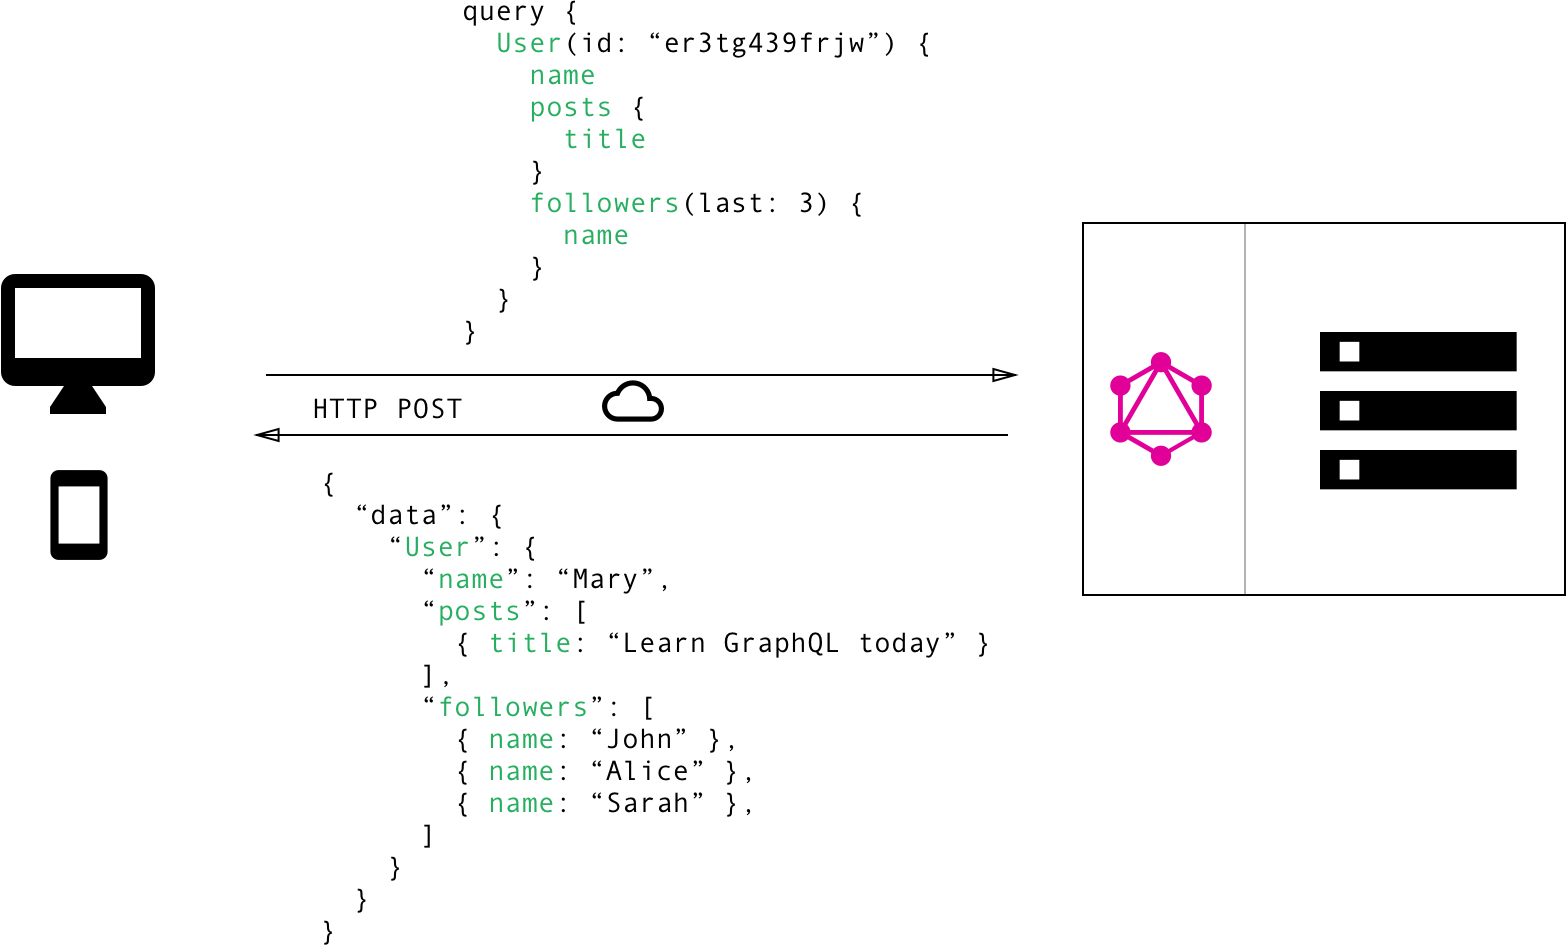
\includegraphics[width=\textwidth]{fetching-graphql.png}
    \caption{How GraphQL solves this problem}
    \label{fig:graphqlFix}
\end{figure}

This is important in our application as in some scenarios where information is being retrieved, we would want to prevent over-fetching. To store trail information, we would need to store a large amount of coordinates per each trail. When a user is searching for a trail initially, we would only require details such as name of the trail, its average rating and so on. Requesting all the coordinates would be a waste at this point and would add extra overhead to the system. 